\section{V\_selector: A rotating velocity selector}
\label{vselector}

\component{V\_selector}{System}{$L_0$, $L_1$, $\omega$, $r_0$, $\phi$, $N$}{}{validated, position is center of input aperture}

\begin{figure}
  \begin{center}
    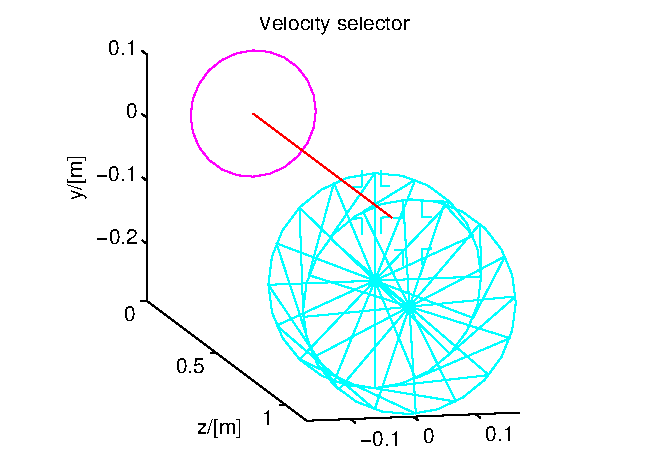
\includegraphics[width=0.9\textwidth]{figures/vselector.eps}
  \end{center}
\caption{A velocity selector}
\label{f:vselector}
\end{figure}

The component {\bf V\_selector} models a rotating velocity
selector constructed from a number of collimator blades
arranged radially on an axis. Two identical slits
at a 12 o'clock position allow
neutron passage at the position of the blades.
The blades are "twisted" on the axis so that a stationary
velocity selector does not transmit any neutrons; the total
twist angle is denoted $\phi$.
By rotating the selector you allow
transmittance of neutrons around certain velocities, given by
\begin{equation}
V_0 = \omega L / \phi ,
\end{equation}
which means that the selector has turned the twist angle
$\phi$ during the neutron flight time $L/V_0$.

Neutrons having a velocity slightly smaller or larger than $V_0$
will either be transmitted or absorbed depending on the exact position
of the rotator blades when the neutron enters the selector.
Assuming this position to be unknown (and assuming infinitely
thin blades), we arrive at
\begin{equation}
T = \left\{
 \begin{array}{ll}
 1 - (N/2\pi ) |\phi-\omega L / V| &
        {\rm if}\,  -1 < (N/2\pi )(\phi -\omega L / V) < 1 \\
    0  &  {\rm otherwise}
 \end{array} \right.
\end{equation}
where $N$ is the number of collimator blades.

A horisontal divergence changes the above formula because of the
angular difference between the entry and exit points of the neutron.
The resulting transmittance resembles the one above, only with
$V$ replaced by $V_z$ and $\phi$ replaced by $(\phi +\psi )$,
where $\psi$ is the angular difference due to
the divergence. An additional vertical divergence does not change
this formula, but it may contribute to $\psi$.
(We have here ignored the very small non-linearity of $\psi$ along the
neutron path in case of both vertical and horisontal divergence).

Adding the effect of a finite blade thickness, $t$, reduces the transmission
by the overall amount
\begin{equation}
dT = (N t) / (2\pi r ) ,
\end{equation}
where $r$ is the distance from the rotation axis. We ignore the variation
of $r$ along the neutron path and use just the average value.

The input parameters for V\_selector are the slit dimensions,
\textit{width}, \textit{height} (in m),
the distance between apertures, $L_0$ (in m), the length of the
collimator blades, $L_1$ (in m), the height from rotation axix to the slit
centre, $r_0$ (in m), the rotation speed $\omega$ (in rpm)
the twist angle $\phi$ (in degrees), the blade thickness $t$ (in m),
and the number of blades, $N$.

The local coordinate system is centered at the slit centre.

